
We have shown that flat minima will bring a better domain generalization. 
In this section, we 
% \jb{first look at existing flatness-aware solvers,}
propose Stochastic Weight Averaging Densely (SWAD) algorithm, and provide empirical quantitative and qualitative analyses on SWAD and flatness to understand why SWAD works better than ERM.

\subsection{A baseline method: stochastic weight averaging}

Since the importance of flatness in loss landscapes has emerged~\cite{keskar2016largebatch,dziugaite2017computing,garipov2018fge,izmailov2018swa,jiang2019fantastic,foret2020sharpness}, several methods have been proposed to find flat minima~\cite{foret2020sharpness,chaudhari2019entropy,izmailov2018swa}. 
We select stochastic weight averaging (SWA)~\cite{izmailov2018swa} as a baseline, which finds flat minima by a weight ensemble approach.
% We adopt stochastic weight averaging (SWA)~\cite{izmailov2018swa} as a our baseline, which is a widely used flatness-aware solver. It finds flat minima by a simple weight ensemble approach. 
% Stochastic weight averaging (SWA)~\cite{izmailov2018swa}, one of the popular approaches, finds flat minima by a simple weight ensemble approach.
% SWA~\cite{izmailov2018swa} is a simple weight ensemble approach to find flat minima. 
More specifically, SWA updates a pretrained model (namely, a model trained with sufficiently enough training epochs, $K_0$) with a cyclical~\cite{smith2017cyclical} or high constant learning rate scheduling. SWA gathers model parameters for every $K$ epochs during the update and averages them for the model ensemble.
SWA finds an ensembled solution of different local optima found by a sufficiently large learning rate to escape a local minimum. \citet{izmailov2018swa} empirically showed that SWA finds flatter minima than ERM. We also considered sharpness-aware minimization (SAM)~\cite{foret2020sharpness}, which is another popular flatness-aware solver, but SWA finds flatter minima than SAM (See Figure~\ref{fig:flatness}).
We illustrate an overview of SWA in Figure~\ref{fig:swa_overview}.
% We examine two widely used flatness-aware solvers: sharpness-aware minimization (SAM)~\cite{foret2020sharpness} and stochastic weight averaging (SWA)~\cite{izmailov2018swa}. SAM approximate robust risk and directly optimize it. SWA averages a number of weights from the end of optimization process. Although SWA does not address flatness in the learning process, they empirically showed that SWA finds flatter minima than ERM. We evaluate flatness-aware solvers by comparing local flatness of the solution found by each algorithm.


% \jb{
% To begin with, we quantify the local flatness of a model parameter $\theta$ by assuming that flat minima will have smaller changes of loss value within its neighborhoods than sharp minima.
% For the given model parameter $\theta$, we compute the expected loss value changes between $\theta$ and parameters on the sphere surrounding $\theta$ with radius $\gamma$, \ie, $\mathcal{F}_\gamma (\theta)=\mathbb {E}_{\| \theta' \| = \|\theta\| + \gamma} [\mathcal{E}(\theta')-\mathcal{E}(\theta)]$.
% In practice, $\mathcal{F}_\gamma(\theta)$ is approximated by Monte-Carlo sampling with 100 samples.
% Note that the proposed local flatness $\mathcal{F}_\gamma(\theta)$ is computationally efficient than measuring curvature using the Hessian-based quantities. Also, $\mathcal{F}_\gamma(\theta)$ has an unbiased finite sample estimator, while the worst-case loss value, \ie, $\max_{\| \theta' \| = \|\theta\| + \gamma}[\mathcal{E}(\theta')-\mathcal{E}(\theta)]$ has no unbiased finite sample estimator.
% As shown in the Figure~\ref{fig:flatness}, this comparison shows SWA finds flatter minima than ERM and SAM.
% }

\subsection{Dense and overfit-aware stochastic weight sampling strategy}
% \vspace{-1em}

\begin{figure}[t]

\centering

% \subcaptionbox{Comparison in loss surface view\label{fig:diff}}{
%     \includegraphics[width=0.27\textwidth]{figures/swa_vs_swad.pdf}
% (a) The extent of flat region depends on the degree of shaking defined as flat. Thanks to constant learning rate and densely averaging, SWAD catches the center of the wider flat region accurately. Relatively, SWA cannot provide enough robustness to domain shifts because it finds a solution in the narrow flat region.
% }\quad
\begin{subfigure}{0.4\linewidth}
    
\includegraphics[width=\linewidth]{figures/swad_concept/conceptfig_legend.pdf}
\end{subfigure}\\
\subcaptionbox{\small SWA\label{fig:swa_overview}}{%
  %\includegraphics[height=3.3cm]
  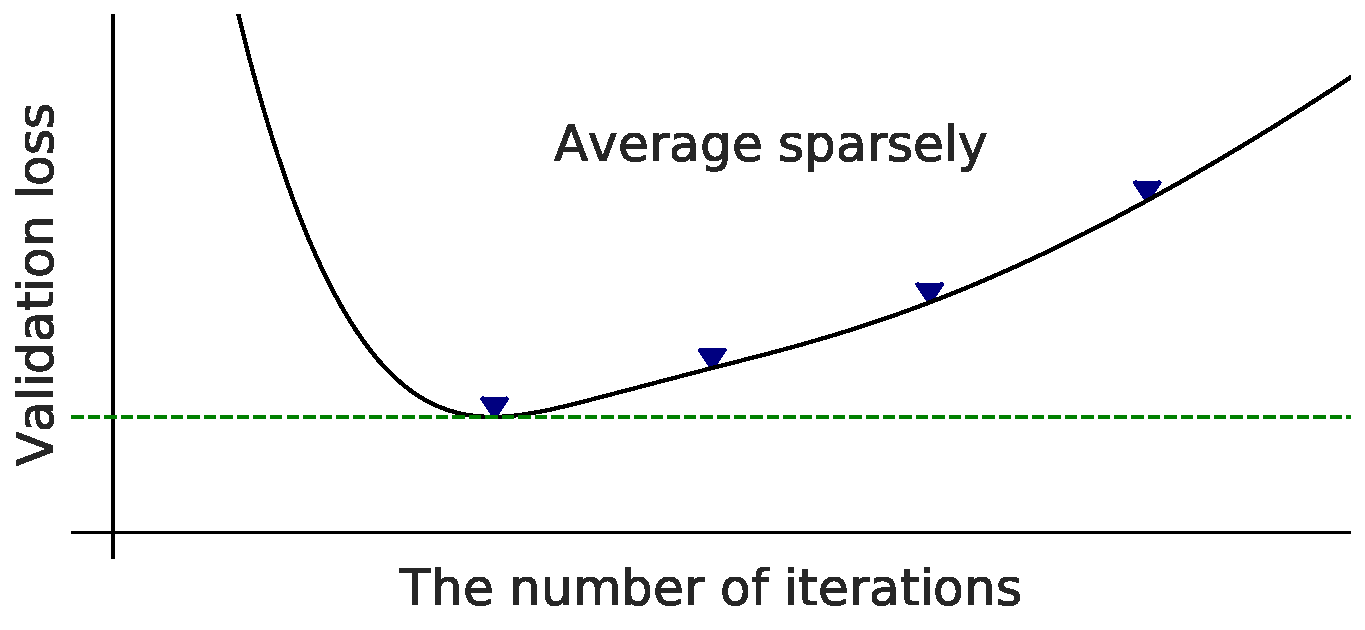
\includegraphics[width=0.4\textwidth]{figures/swad_concept/swa_concept_fig.pdf}%
}
\qquad \quad
\subcaptionbox{\small SWAD\label{fig:swad_overview} (proposed)}{%
  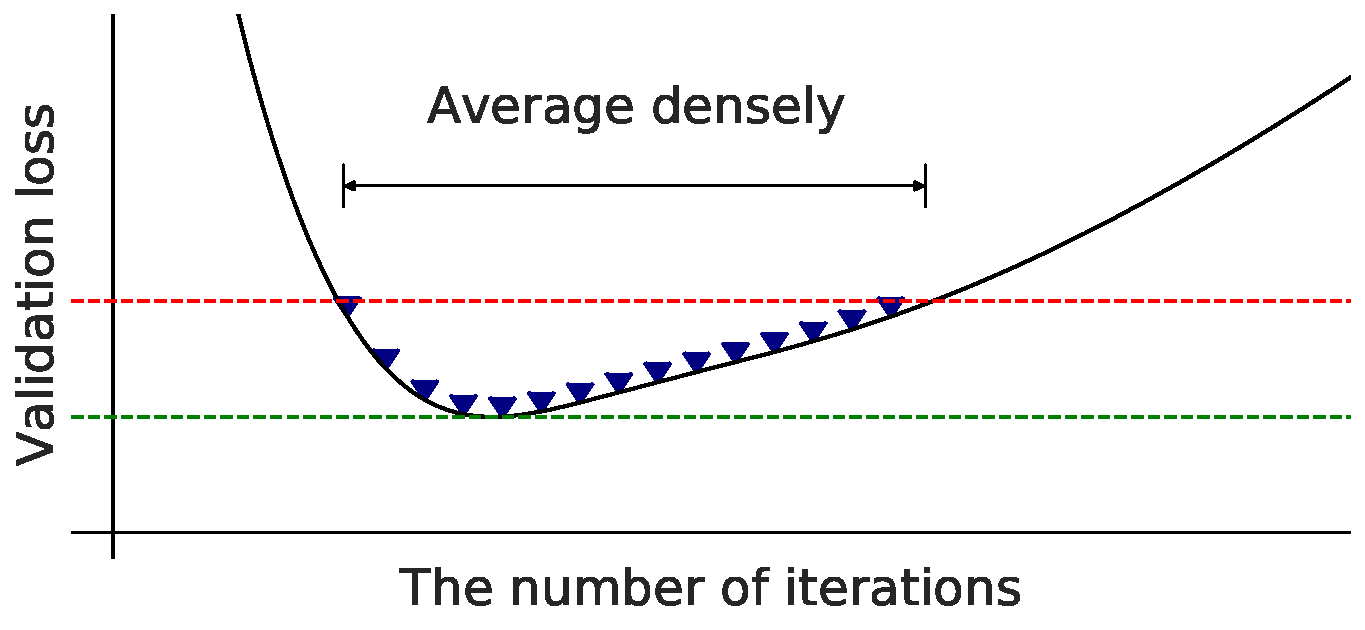
\includegraphics[width=0.4\textwidth]{figures/swad_concept/swad_concept_fig.pdf}%
}
\vspace{-.5em}
\caption{\small {\bf Comparison between SWA and SWAD.} (a) SWA collects stochastic weights for every $K$ epochs from the pre-defined $K_0$ epochs to the final epoch.
% in an interval of certain epoch. 
(b) Our SWAD collects stochastic weights \textbf{\textit{densely}}, \ie, for every iteration, to obtain sufficiently many weights. SWAD collects the weights from the start iteration $t_s$ to the end iteration $t_e$, where $t_s$ and $t_e$ are obtained by monitoring the validation loss (\textbf{\textit{overfit-aware}} scheduling).
% By the proposed dense and overfit-aware gathering strategy, SWAD can collect sufficiently many stochastic weights while avoiding overfitting.
% (b) SWAD computes a threshold from the minimum validation loss, chooses a range from the threshold, and averages all of the weight in the range.}
}
\label{fig:swa_swad_comparison}
\vspace{-1.5em}
\end{figure}

% \jb{TODO: update below paragraph to fit in with above added subsection}

% \jb{Based on the flatness analysis, we choose SWA as our baseline flatness-aware solver.}
% SWA~\cite{izmailov2018swa} is a simple weight ensemble approach to find flat minima. More specifically, SWA updates a pretrained model (namely, a model trained with sufficiently enough training epochs, $K_0$) with a cyclical~\cite{smith2017cyclical} or high constant learning rate scheduling. SWA gathers model parameters for every $K$ epochs during the update and averages them for the model ensemble.
% Intuitively, SWA finds a solution that is an ensemble of different local optima found by a sufficiently large learning rate to escape a local minimum.
% We illustrate an overview of SWA in Figure~\ref{fig:swa_overview}.
%SWA has advantages over other flatness-aware methods~\cite{chaudhari2019entropy, foret2020sharpness} in that it does not change the objective function to penalize sharp minima and does not require any additional computation for sharpness related quantities.

% Comparing to other flatness-aware methods~\cite{chaudhari2019entropy, foret2020sharpness}, SWA does not change the objective function by penalizing sharp minima, and no additional computation for sharpness related quantities is needed.

% However, in practice, we observe that directly applying the vanilla SWA to domain generalization tasks often suffers from the overfitting issue.
% From this motivation, we propose a modified SWA, named SWA-densely (SWAD).

% How about this flow?
% 1) learning from multiple source domains -> wider variance of empirical risks on mini-batches. (See Figure 5) 
% 2) to gather diverse model weights, SWAD gathers weights densely

% Despite its advantages, we find that there are two problems to apply SWA to domain generalization task directly.
% SWA has two major drawbacks. 
Despite its advantages, directly applying SWA to DG task has two problems.
First, SWA averages a few weights (usually less than ten) by sampling weights for every $K$ epochs, results in an inaccurate approximation of flat minima on a high-dimensional parameter space (\eg, 23M for ResNet-50~\cite{he2016_cvpr_resnet}).
% \footnote{\citet{izmailov2018swa} also observed similar phenomenon: averaging 10 weights outperforms 5 weights.}
Furthermore, a common DG benchmark protocol uses relatively small training epochs (\eg,
% DomainBed~\cite{gulrajani2020domainbed} typically trained with less than two epochs, 
\citet{gulrajani2020domainbed} trained with less than two epochs for \data{DomainNet} benchmark), resulting in insufficient stochastic weights for SWA.
% not a sufficient to gather stochastic weights for SWA.
From this motivation, we propose a \textbf{\textit{``dense''}} sampling strategy for gathering sufficiently enough stochastic weights.

In addition, widely used DG datasets, such as \data{PACS} ($\approx$ 10K images, 7 classes) and \data{VLCS} ($\approx$ 11K images, 5 classes), are relatively smaller than large-scale datasets, such as ImageNet~\cite{russakovsky2015imagenet} ($\approx$ 1.2M images, 1K classes). In this case, we observe that a simple ERM approach is rapidly reached to a local optimum only within a few epochs, and easily suffers from the overfitting issue, \ie, the validation loss is increased after a few training epochs.
% In addition, since domain generalization benchmarks, such as \data{PACS} ($\approx$ 10K images, 4 domains, 7 classes), \data{VLCS} ($\approx$ 11K images, 4 domains, 5 classes), \data{OfficeHome} ($\approx$ 15K images, 4 domains, 65 classes), and \data{TerraIncognita} ($\approx$ 25K images, 4 domains, 10 classes), are relatively smaller datasets than large-scale datasets, such as ImageNet~\cite{russakovsky2015imagenet} ($\approx$ 1.2M images, 1K classes), we observe that a simple ERM approach is rapidly reached to a local optimum only within a few epochs, and easily suffers from the overfitting issue, \ie, the validation loss is increased after a few training epochs.
It implies that directly applying the vanilla SWA will suffer from the overfitting issue by averaging sub-optimal solutions (\ie, overfitted parameters).
Hence, we need an \textbf{\textit{``overfit-aware''}} sampling scheduling to omit the sub-optimal solutions for SWA.

The main idea of Stochastic Weight Averaging Densely (SWAD) is a dense and overfit-aware stochastic weight gathering strategy.
First, instead of collecting weights for every $K$ epochs, SWAD collects weights for every iteration. This dense sampling strategy easily collects sufficiently many weights than the sparse one.
% (for every $K$ epochs).
We also employ overfit-aware sampling scheduling by considering traces of the validation loss.
Instead of sampling weights from $K_0$ pretraining epochs to the final epoch, we search the start iteration (when the validation loss achieves a local optimum for the first time) and the end iteration (when the validation loss is no longer decreased, but keep increasing).
More specifically, we introduce three parameters: an optimum patient parameter $N_s$, an overfitting patient parameter $N_e$, and the tolerance rate $r$ for searching the start iteration $t_s$ and the end iteration $t_e$.
First, we search $t_s$ which satisfies $\min_{i\in[0, \ldots, N_s-1]} \mathcal E_\text{val}^{(t_s + i)}=\mathcal E_\text{val}^{(t_s)}$, where $\mathcal{E}_\text{val}^{(i)}$ denotes the validation loss at iteration $i$.
Simply, $t_s$ is the first iteration where the loss value is no longer decreased during $N_s$ iterations.
Then, we find $t_e$ satisfying $\min_{i \in [0, 1, \ldots, N_e - 1]} \mathcal E_\text{val}^{(t_e + i)} > r \mathcal E_\text{val}^{(t_s)}$.
In other words, $t_e$ is the first iteration where the validation loss values exceed the tolerance $r$ during $N_e$ iterations.


We illustrate the overview of SWAD and the comparison of SWAD to SWA in Figure~\ref{fig:swa_swad_comparison}. Detailed pseudo code is provided in Appendix B.4.
We compare SWAD with other possible SWA strategies in \S\ref{label:s__ablation} and show that our design choice works better for DG tasks.

\subsection{Empirical analysis of SWAD and flatness}
\label{subsection:s__empirical_analysis_of_swad_and_flatness}

% \input{figures/flatness_comparison}
% \input{figures/flatness_comparison_w_avg}

\begin{figure}[t]
    \centering
    % \vspace{-0.5em}
    \setlength{\tabcolsep}{0pt}
    \newcommand\figwidth{.24}
    % \renewcommand{\arraystretch}{1.5}
    \begin{subfigure}{0.55\linewidth}
        
\includegraphics[width=\linewidth]{figures/flatness/legend.pdf}
    \end{subfigure}\\
    %
    % \begin{subfigure}{1.0\linewidth}
        \centering
        \begin{subfigure}{0.3\linewidth}
            \setlength{\abovecaptionskip}{3pt}
            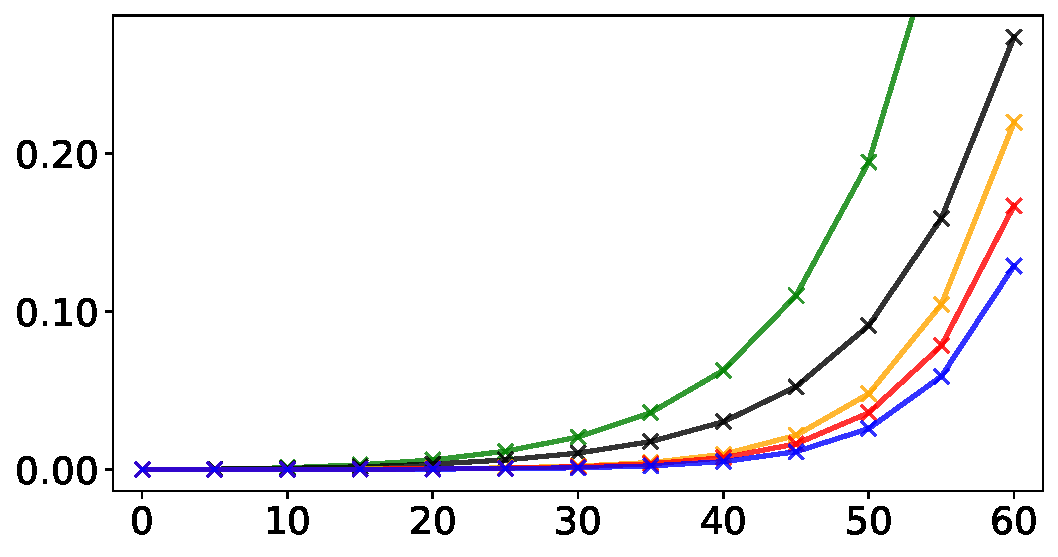
\includegraphics[width=\linewidth]{figures/flatness/PACS_TE4_Train_S5_MD60_N100_BNFalse.pdf}
            \caption{Average train flatness}
        \end{subfigure}
        \quad
        \begin{subfigure}{0.3\linewidth}
            \setlength{\abovecaptionskip}{3pt}
            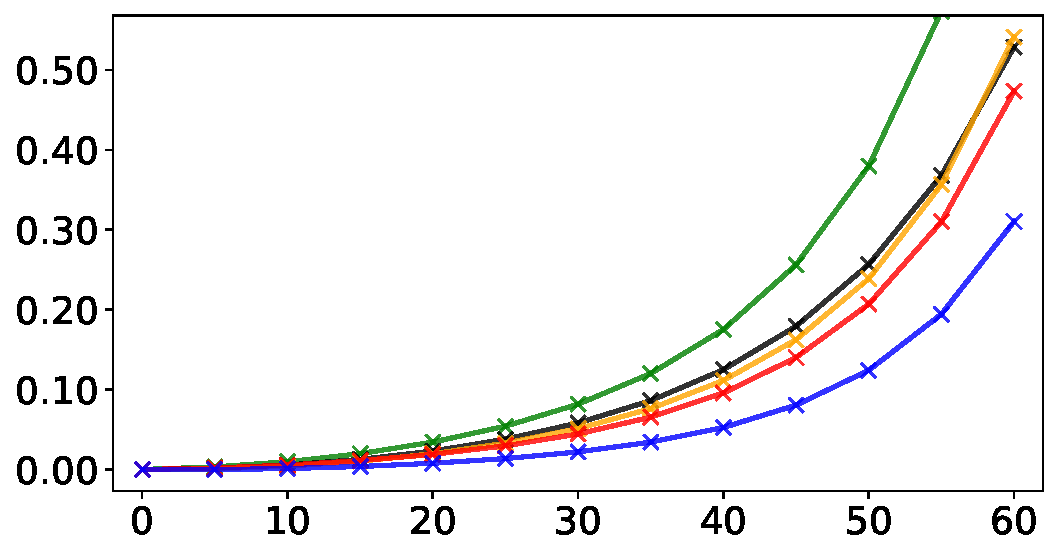
\includegraphics[width=\linewidth]{figures/flatness/PACS_TE4_Test_S5_MD60_N100_BNFalse.pdf}
            \caption{Average test flatness}
        \end{subfigure}
    %     \caption{\small Averaged flatness on \data{PACS} dataset. Left and right figures indicate averaged train and test flatness, respectively.}
    % \end{subfigure}
    \\\vspace{0.4em}
    \begin{subfigure}{1.0\linewidth}
        \begin{tabular*}{\textwidth}{c @{\extracolsep{\fill}} cccc}
            \rotatebox[origin=c]{90}{Train}
            &
            \raisebox{-0.45\height}{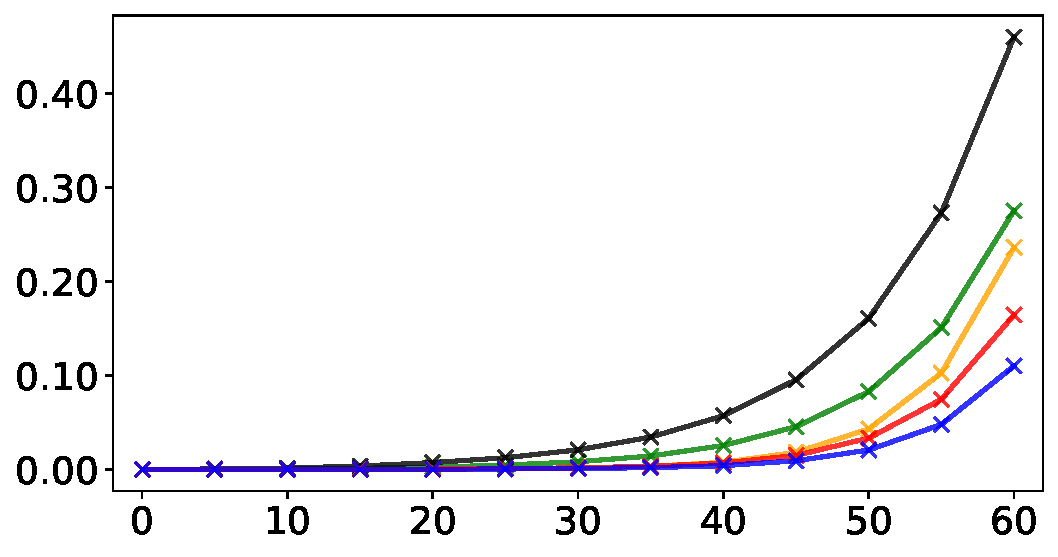
\includegraphics[width=\figwidth\textwidth]{figures/flatness/PACS_TE0_Train_S5_MD60_N100_BNFalse.pdf}}
            &
            \raisebox{-0.45\height}{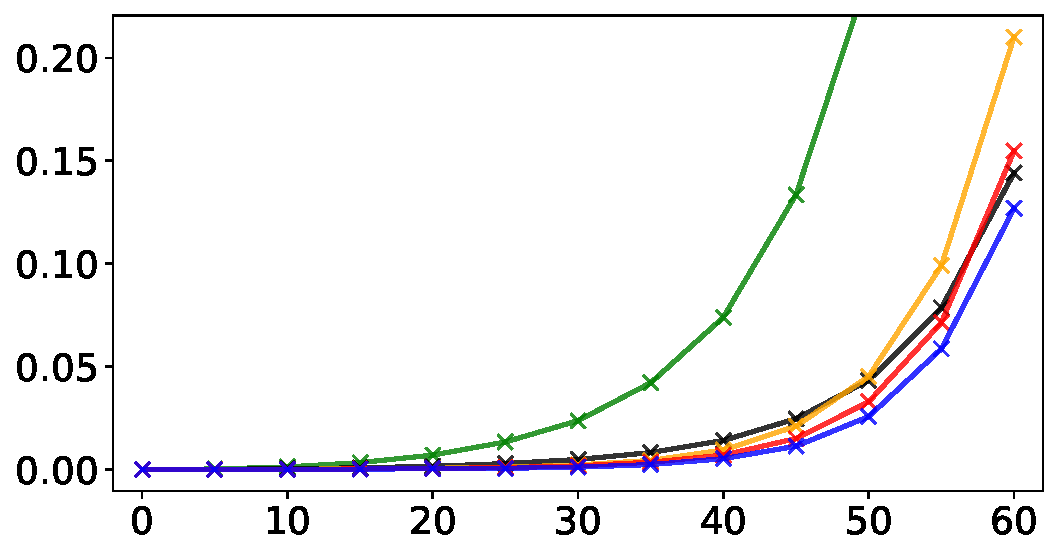
\includegraphics[width=\figwidth\textwidth]{figures/flatness/PACS_TE1_Train_S5_MD60_N100_BNFalse.pdf}}
            &
            \raisebox{-0.45\height}{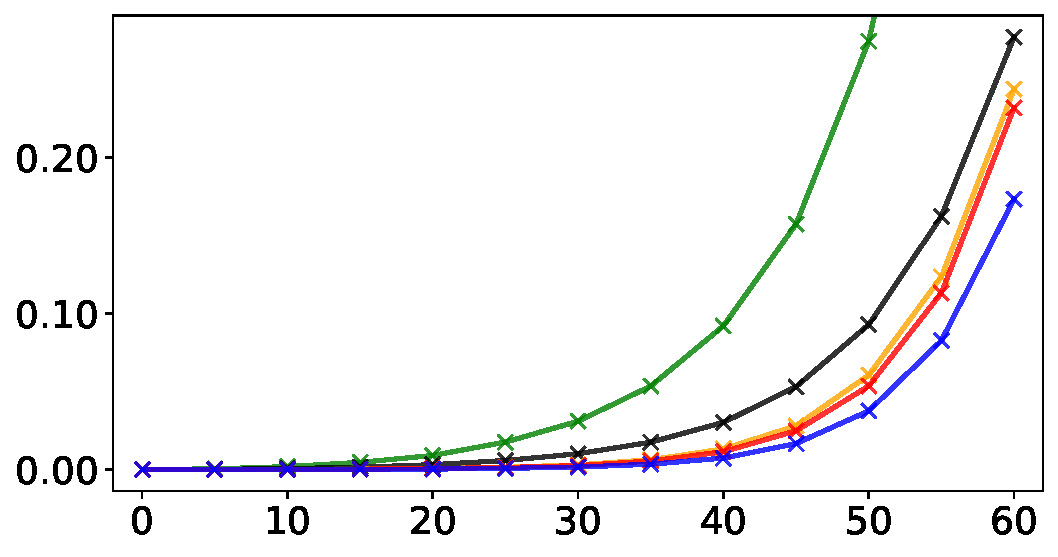
\includegraphics[width=\figwidth\textwidth]{figures/flatness/PACS_TE2_Train_S5_MD60_N100_BNFalse.pdf}}
            &
            \raisebox{-0.45\height}{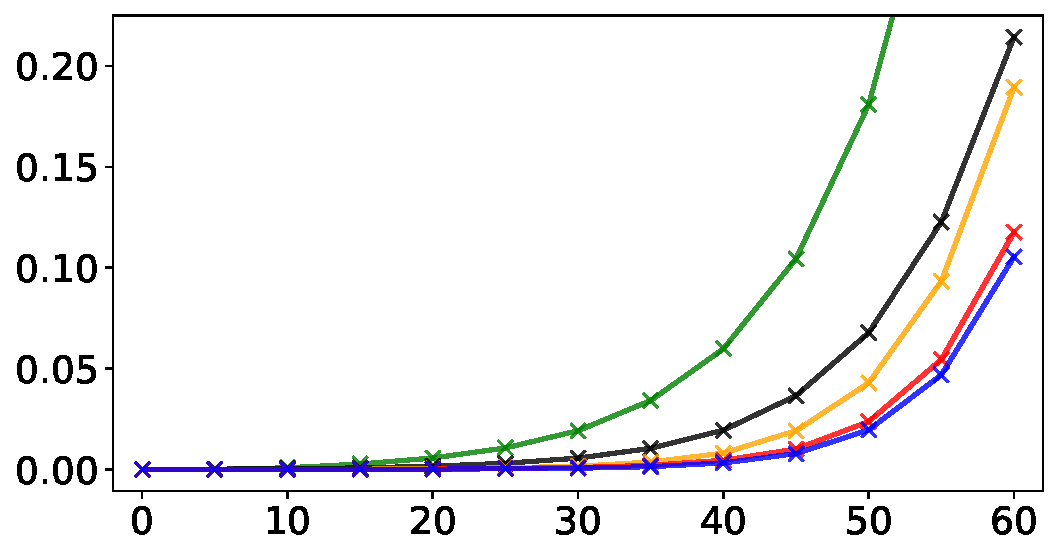
\includegraphics[width=\figwidth\textwidth]{figures/flatness/PACS_TE3_Train_S5_MD60_N100_BNFalse.pdf}}
        \\
            \rotatebox[origin=c]{90}{Test}
            &
            \raisebox{-0.5\height}{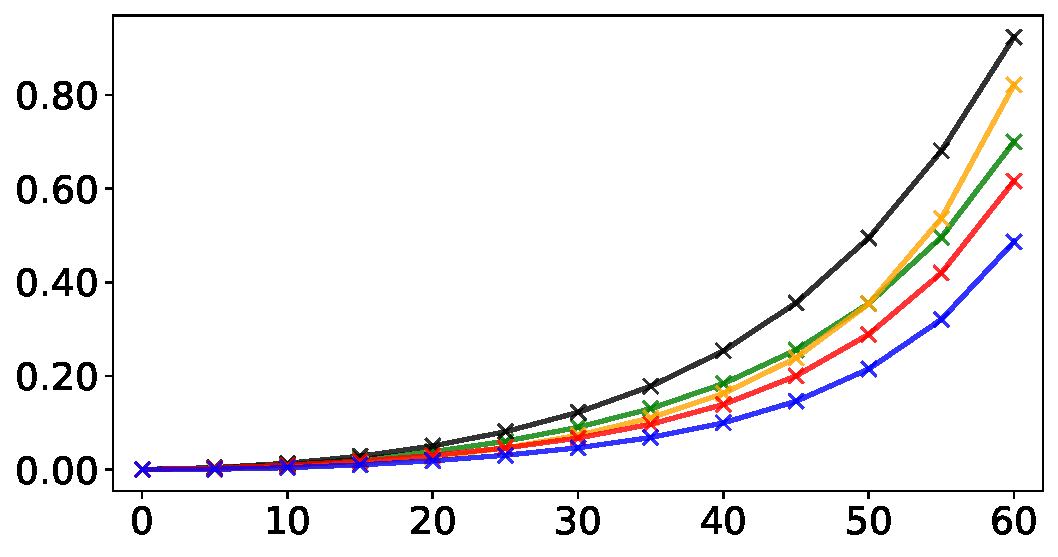
\includegraphics[width=\figwidth\textwidth]{figures/flatness/PACS_TE0_Test_S5_MD60_N100_BNFalse.pdf}}
            &
            \raisebox{-0.5\height}{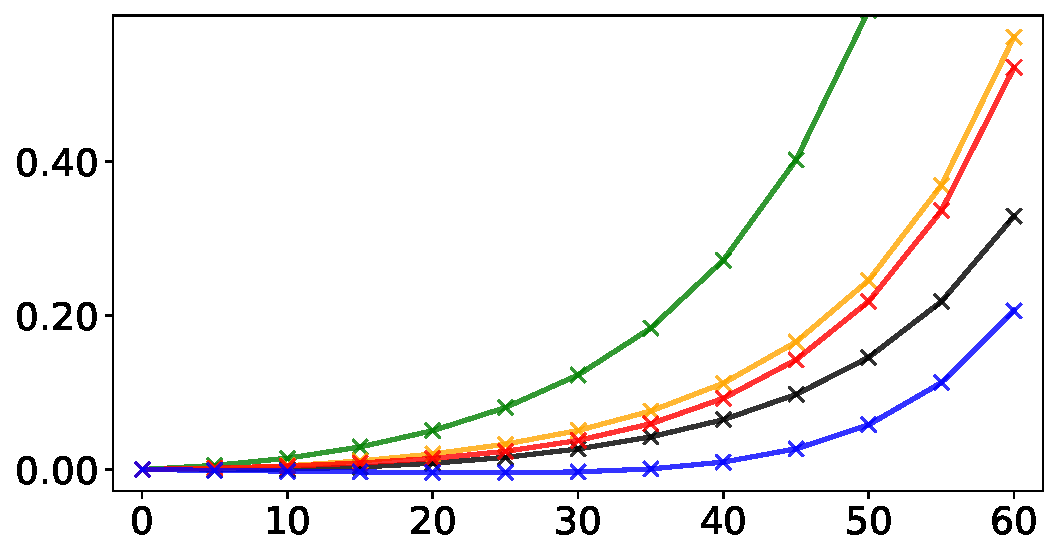
\includegraphics[width=\figwidth\textwidth]{figures/flatness/PACS_TE1_Test_S5_MD60_N100_BNFalse.pdf}}
            &
            \raisebox{-0.5\height}{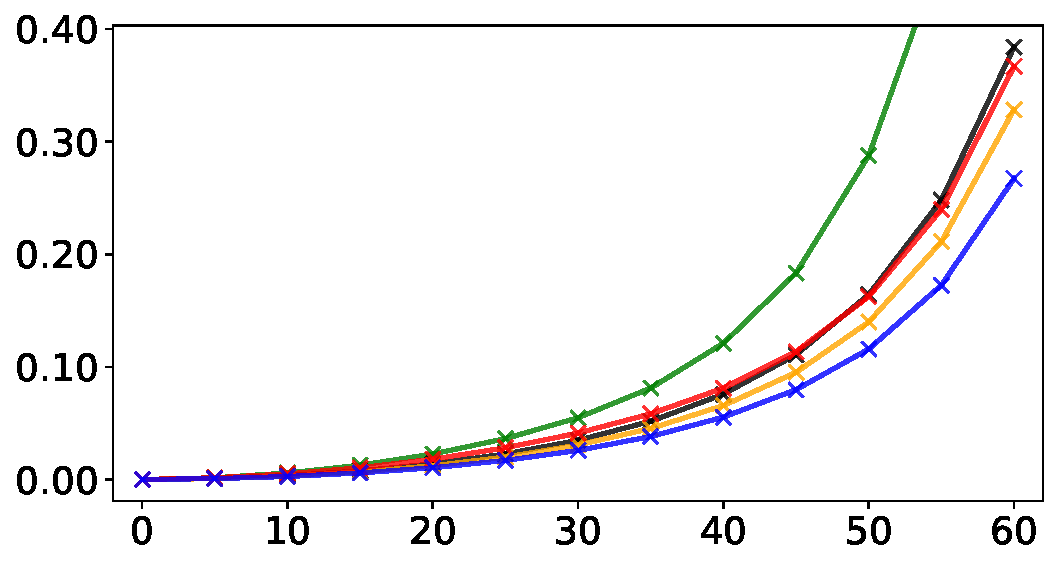
\includegraphics[width=\figwidth\textwidth]{figures/flatness/PACS_TE2_Test_S5_MD60_N100_BNFalse.pdf}}
            &
            \raisebox{-0.5\height}{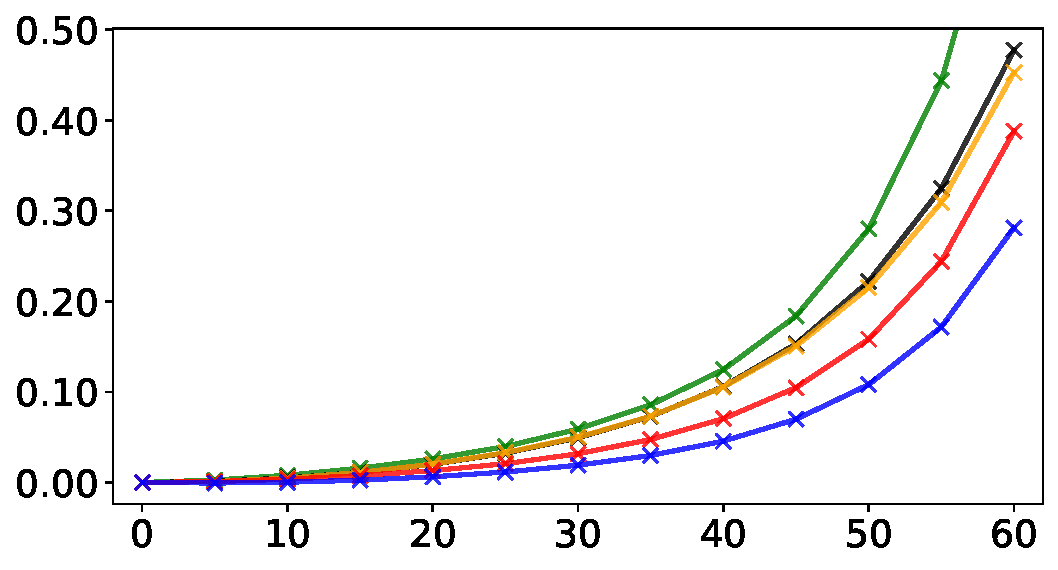
\includegraphics[width=\figwidth\textwidth]{figures/flatness/PACS_TE3_Test_S5_MD60_N100_BNFalse.pdf}}
        \\
            &
            {\small \textit{Art painting} (test)}
            &
            {\small \textit{Cartoon} (test)}
            &
            {\small \textit{Photo} (test)}
            &
            {\small \textit{Sketch} (test)}
        \end{tabular*}
        \setlength{\abovecaptionskip}{3pt}
        \caption{\small Flatness for each target domain}
    \end{subfigure}
    \caption{\small \textbf{Local flatness comparisons.} We plot the local flatness via loss gap, \ie, $\mathcal{F}_\gamma(\theta)=\mathbb {E}_{\| \theta' \| = \|\theta\| + \gamma} [\mathcal{E}(\theta')-\mathcal{E}(\theta)]$, of ERM, SAM, SWA, and SWAD by varying radius $\gamma$ on different domains of \data{PACS} dataset. For each figure, Y-axis indicates the flatness $\mathcal{F}_\gamma(\theta)$ and X-axis indicates the radius $\gamma$. We measure the train flatness $\mathcal{F_\gamma^D}(\theta)$ on seen domains and the test flatness $\mathcal{F_\gamma^T}(\theta)$ on unseen domain. Each point is computed by Monte-Carlo approximation with 100 random samples. This comparisons show SWAD finds flatter minima than not only ERM but also SAM and SWA.
    %, in both train and test domains.
    }
    \label{fig:flatness}
\vspace{-1em}
\end{figure}


Here, we analyze solutions found by SWAD in terms of flatness. We first verify that the SWAD solution is flatter than those of ERM, SWA, and SAM. Our loss surface visualization shows that the SWAD solution is located on the center of the flat region, while ERM finds a boundary solution.
Finally, we show that the sharp boundary solutions by ERM are not generalized well, resulting in sensitivity to the model selection.
All following empirical analyses are conducted on \data{PACS} dataset, validating by all four domains (art painting, cartoon, photo, and sketch).

\paragraph{Local flatness anaylsis.}
% We verify that the proposed SWAD finds flatter minima than ERM and SWA.

To begin with, we quantify the local flatness of a model parameter $\theta$ by assuming that flat minima will have smaller changes of loss value within its neighborhoods than sharp minima.
For the given model parameter $\theta$, we compute the expected loss value changes between $\theta$ and parameters on the sphere surrounding $\theta$ with radius $\gamma$, \ie, $\mathcal{F}_\gamma (\theta)=\mathbb {E}_{\| \theta' \| = \|\theta\| + \gamma} [\mathcal{E}(\theta')-\mathcal{E}(\theta)]$.
In practice, $\mathcal{F}_\gamma(\theta)$ is approximated by Monte-Carlo sampling with 100 samples.
Note that the proposed local flatness $\mathcal{F}_\gamma(\theta)$ is computationally efficient than measuring curvature using the Hessian-based quantities. Also, $\mathcal{F}_\gamma(\theta)$ has an unbiased finite sample estimator, while the worst-case loss value, \ie, $\max_{\| \theta' \| = \|\theta\| + \gamma}[\mathcal{E}(\theta')-\mathcal{E}(\theta)]$ has no unbiased finite sample estimator.

In Figure~\ref{fig:flatness}, we compare $\mathcal{F}_\gamma(\theta)$ of ERM, SAM, SWA with cyclic learning rate, SWA with constant learning rate, and SWAD by varying radius $\gamma$.
% The solution found by SWA and SWAD shows lower local flatness quantities than ERM in all experiments.
SAM and SWA find the solutions with lower local flatness than ERM on average.
SWAD finds the most flat minimum in every experiment.
% We also observe that our dense and overfit-aware sampling strategy, \ie, SWAD, finds flatter optima than SWA and SAM does.


\begin{figure}[tb]
\begin{center}
\setlength{\tabcolsep}{0pt}
\newcommand\figwidth{.22}
%
\begin{tabular*}{0.92\textwidth}{c @{\extracolsep{\fill}} cccc}
    \rotatebox[origin=c]{90}{Train}
    &
    \raisebox{-0.45\height}{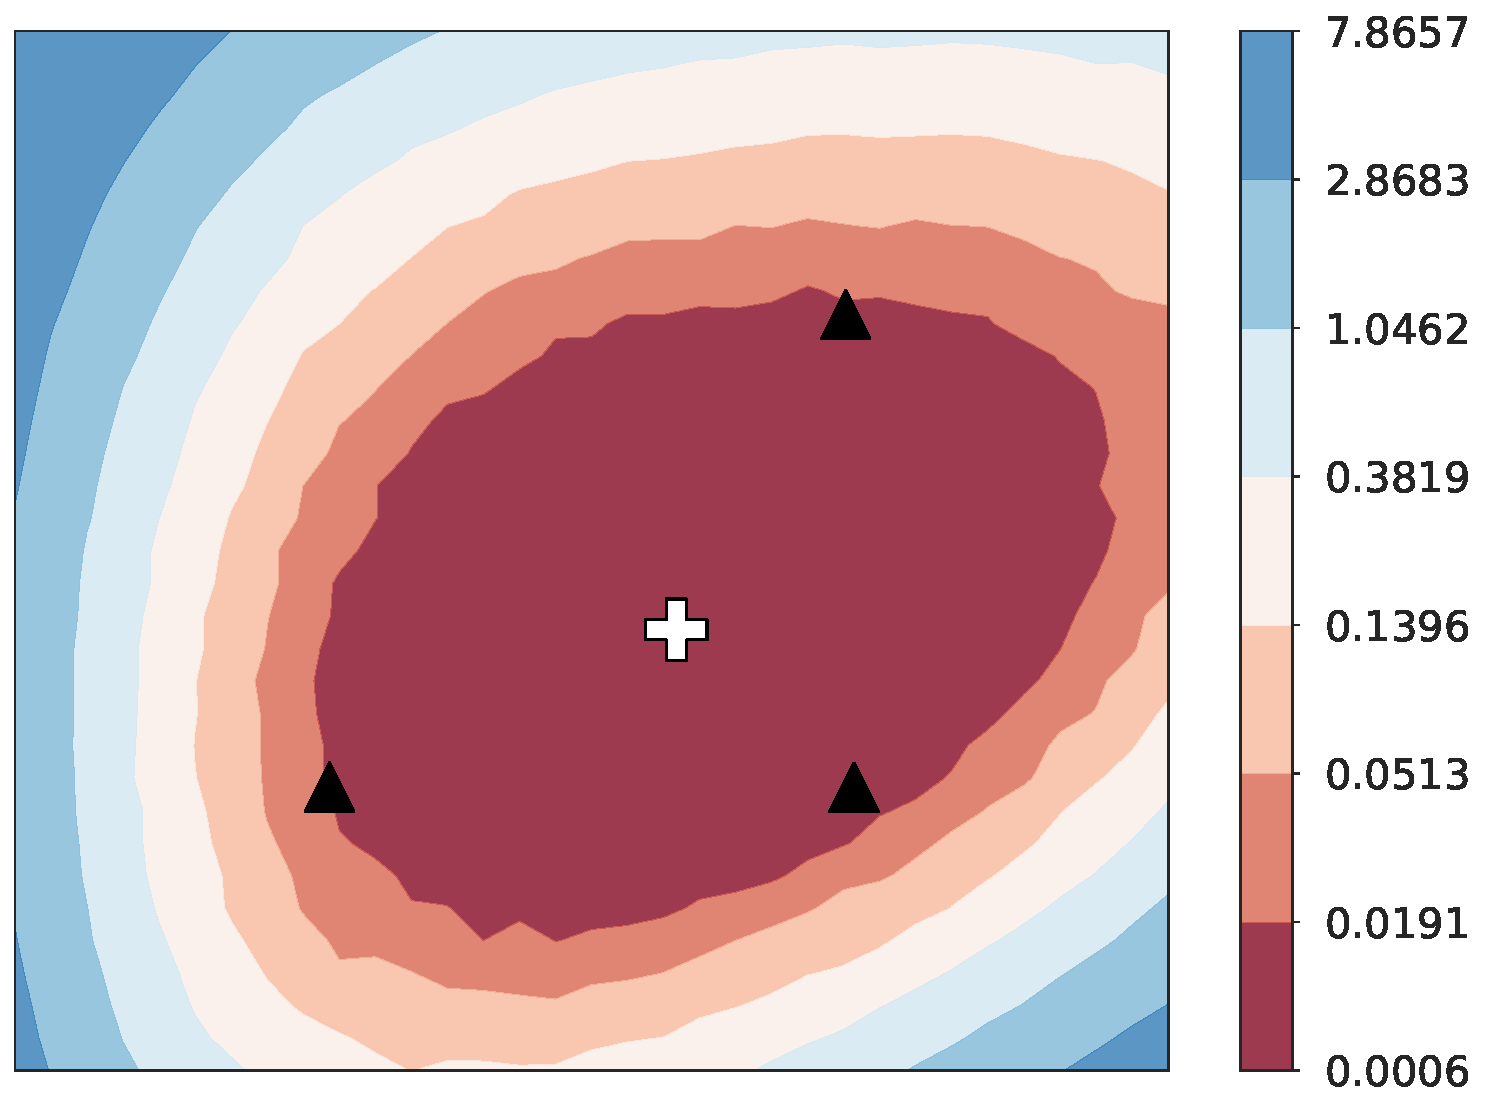
\includegraphics[width=\figwidth\textwidth]{figures/loss_surfaces/TE0_in_loss_plane.pdf}}
    &
    \raisebox{-0.45\height}{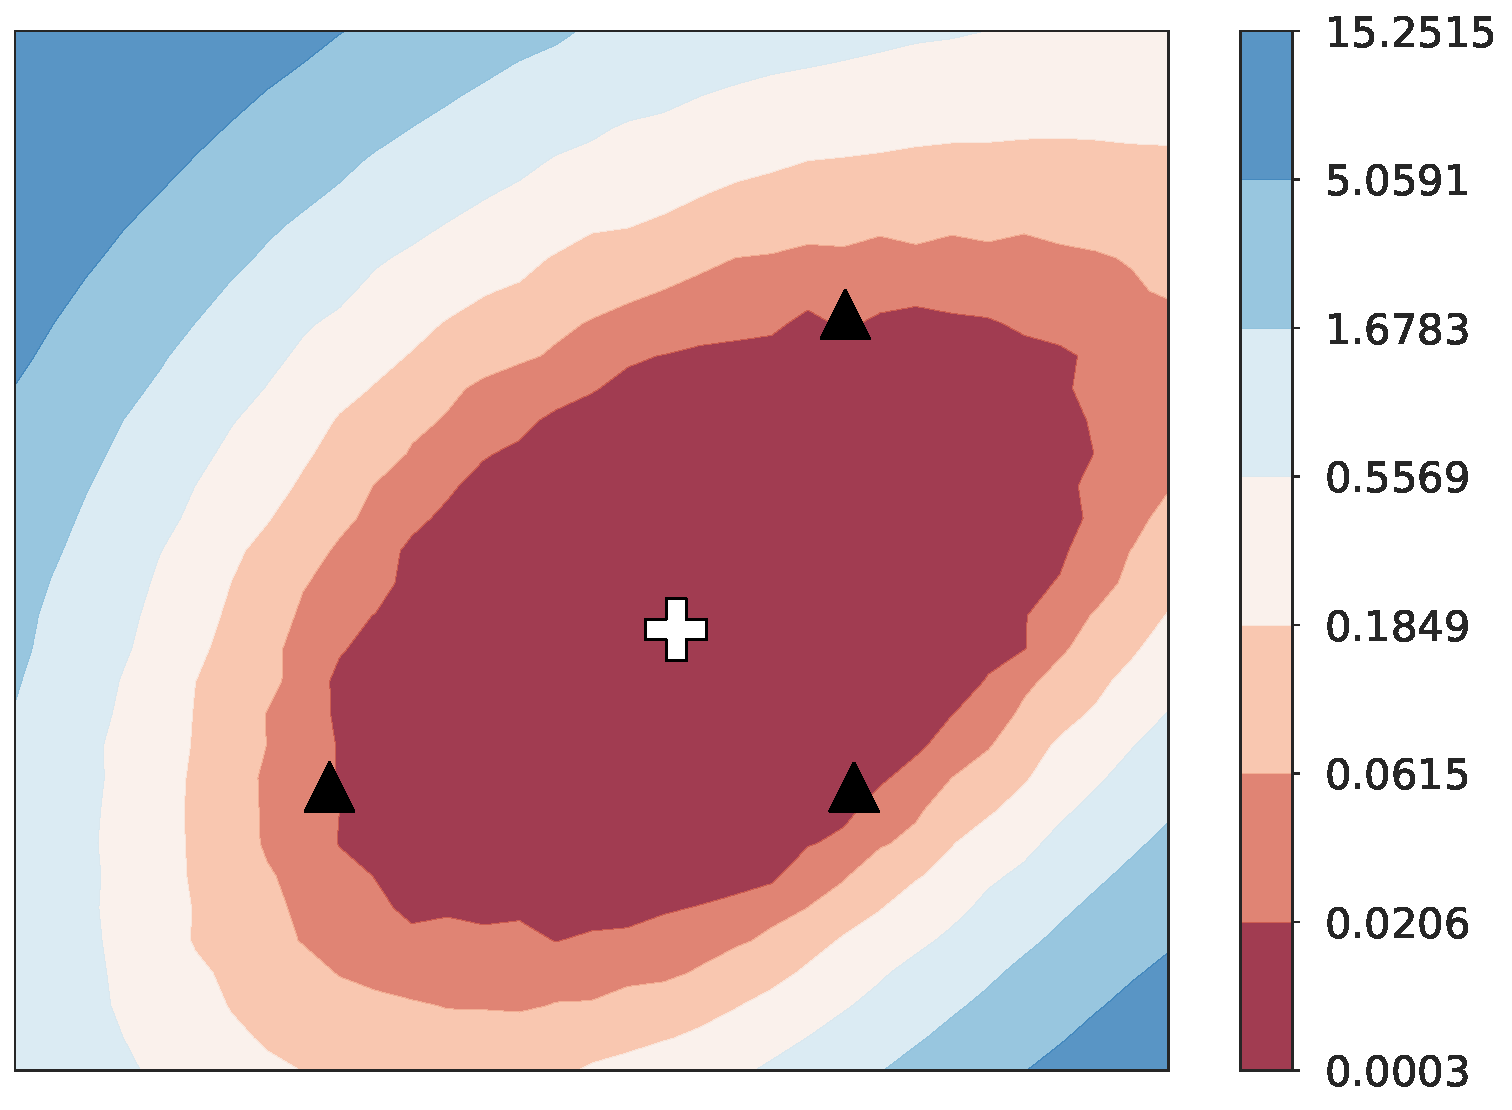
\includegraphics[width=\figwidth\textwidth]{figures/loss_surfaces/TE1_in_loss_plane.pdf}}
    &
    \raisebox{-0.45\height}{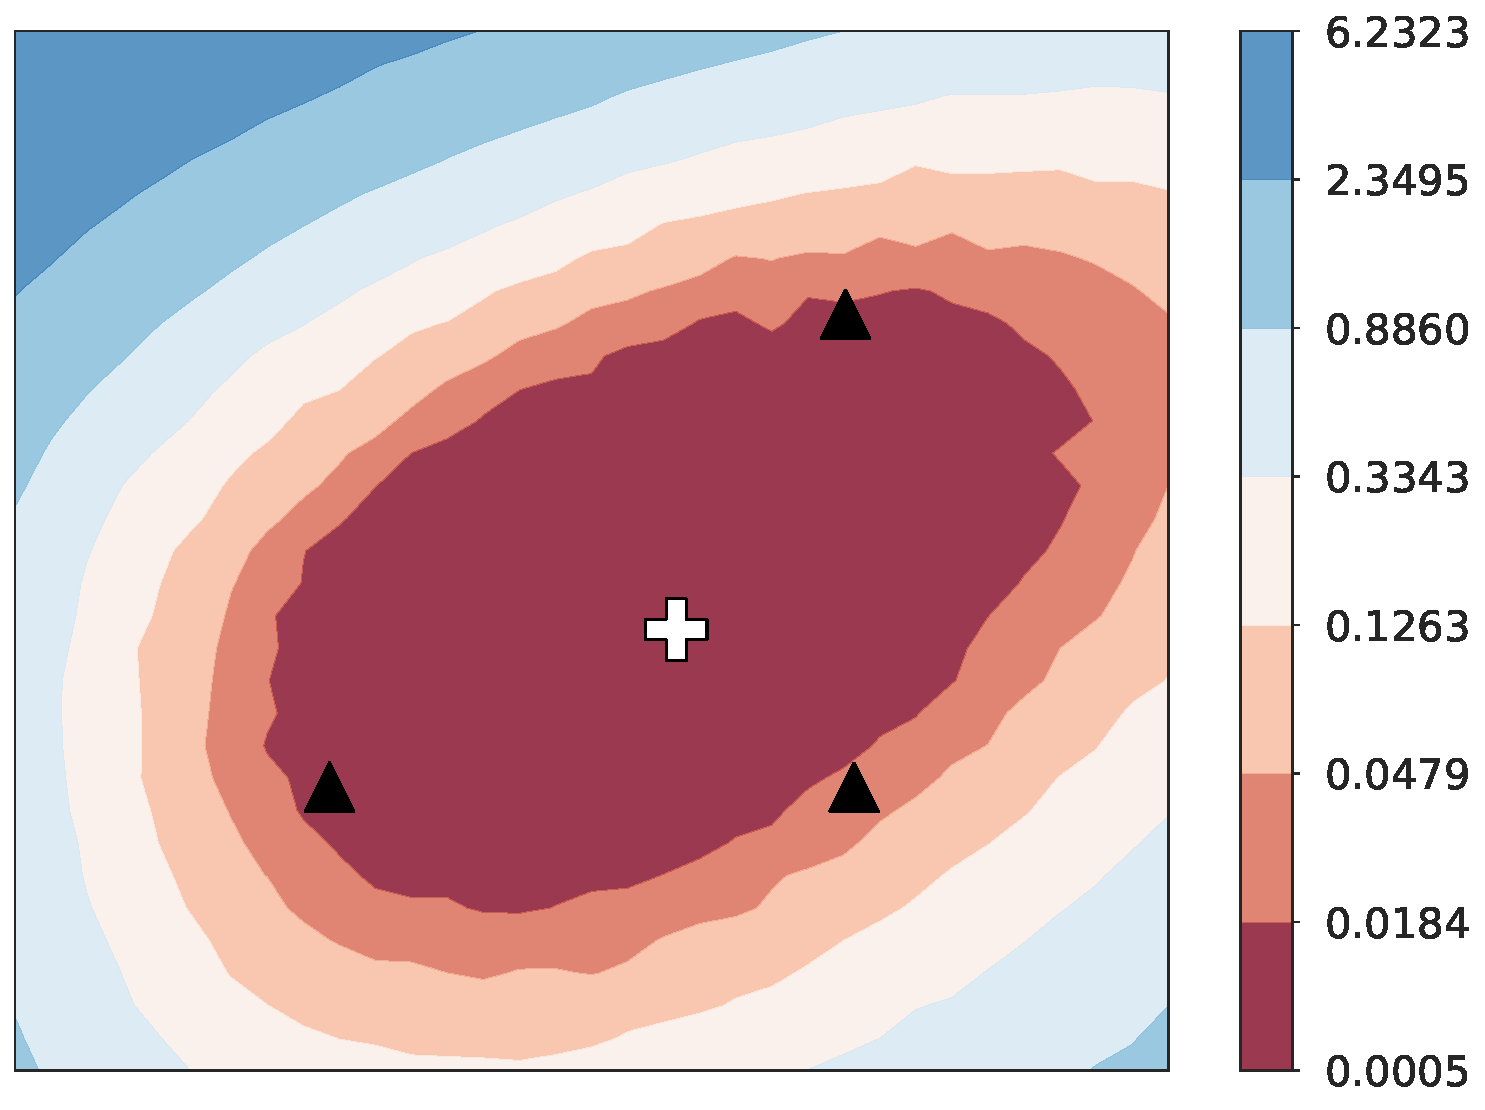
\includegraphics[width=\figwidth\textwidth]{figures/loss_surfaces/TE2_in_loss_plane.pdf}}
    &
    \raisebox{-0.45\height}{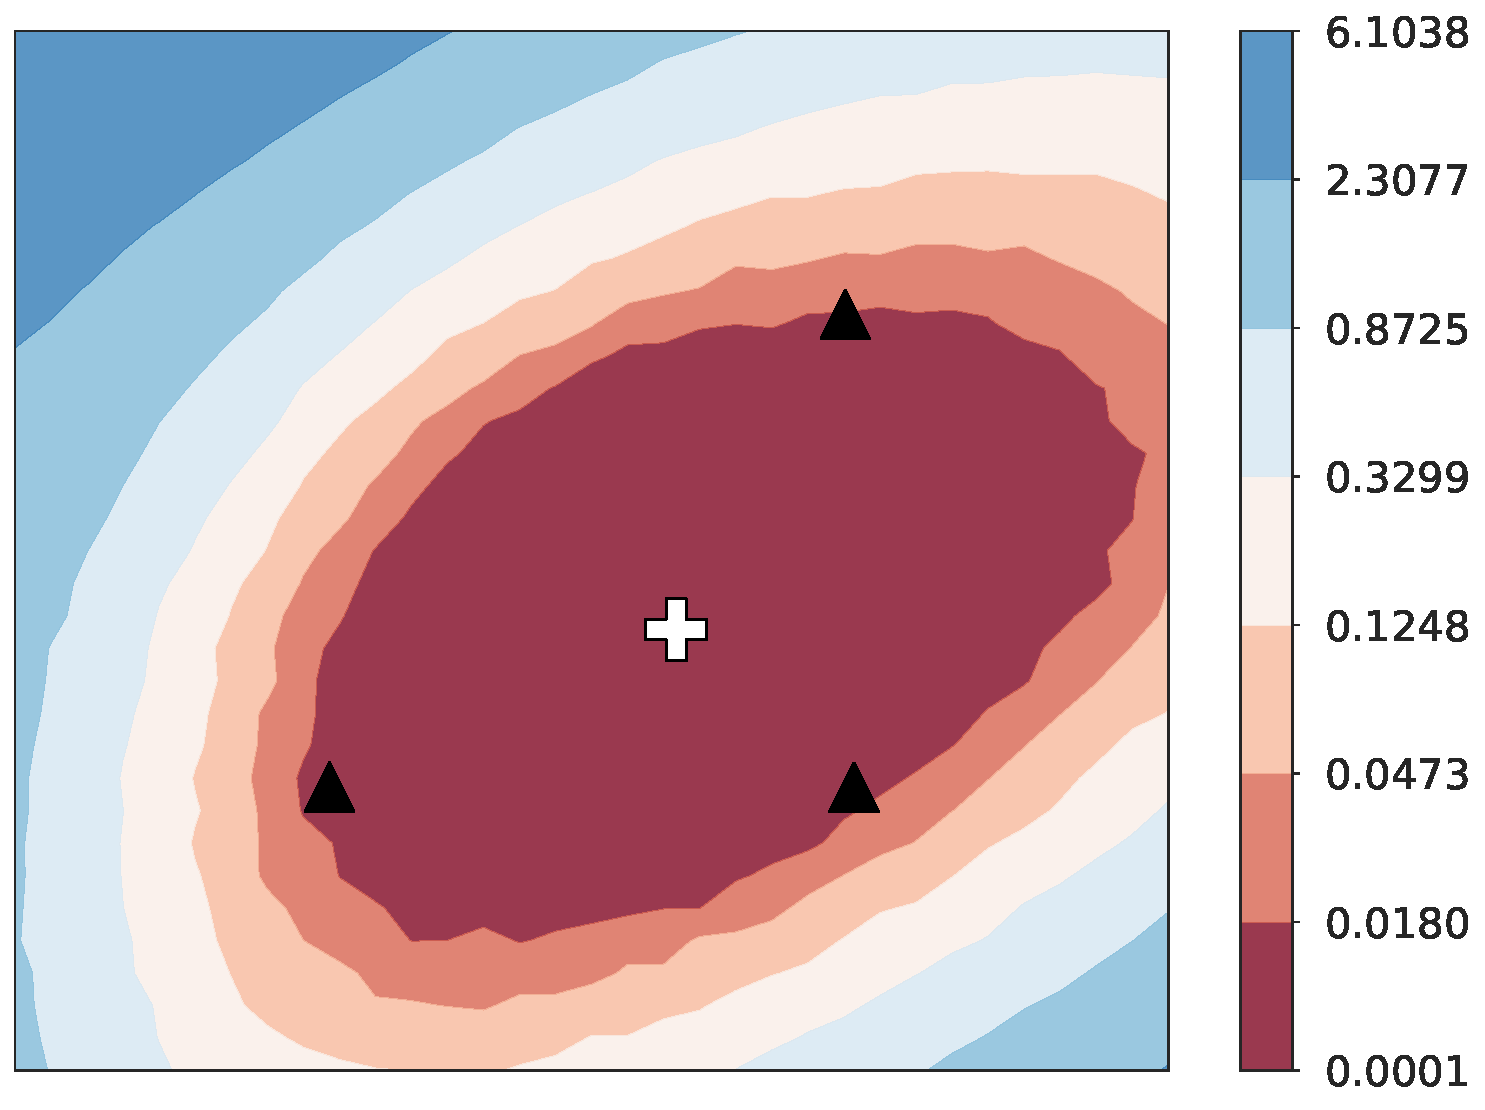
\includegraphics[width=\figwidth\textwidth]{figures/loss_surfaces/TE3_in_loss_plane.pdf}}
\\
    \rotatebox[origin=c]{90}{Test}
    &
    \raisebox{-0.5\height}{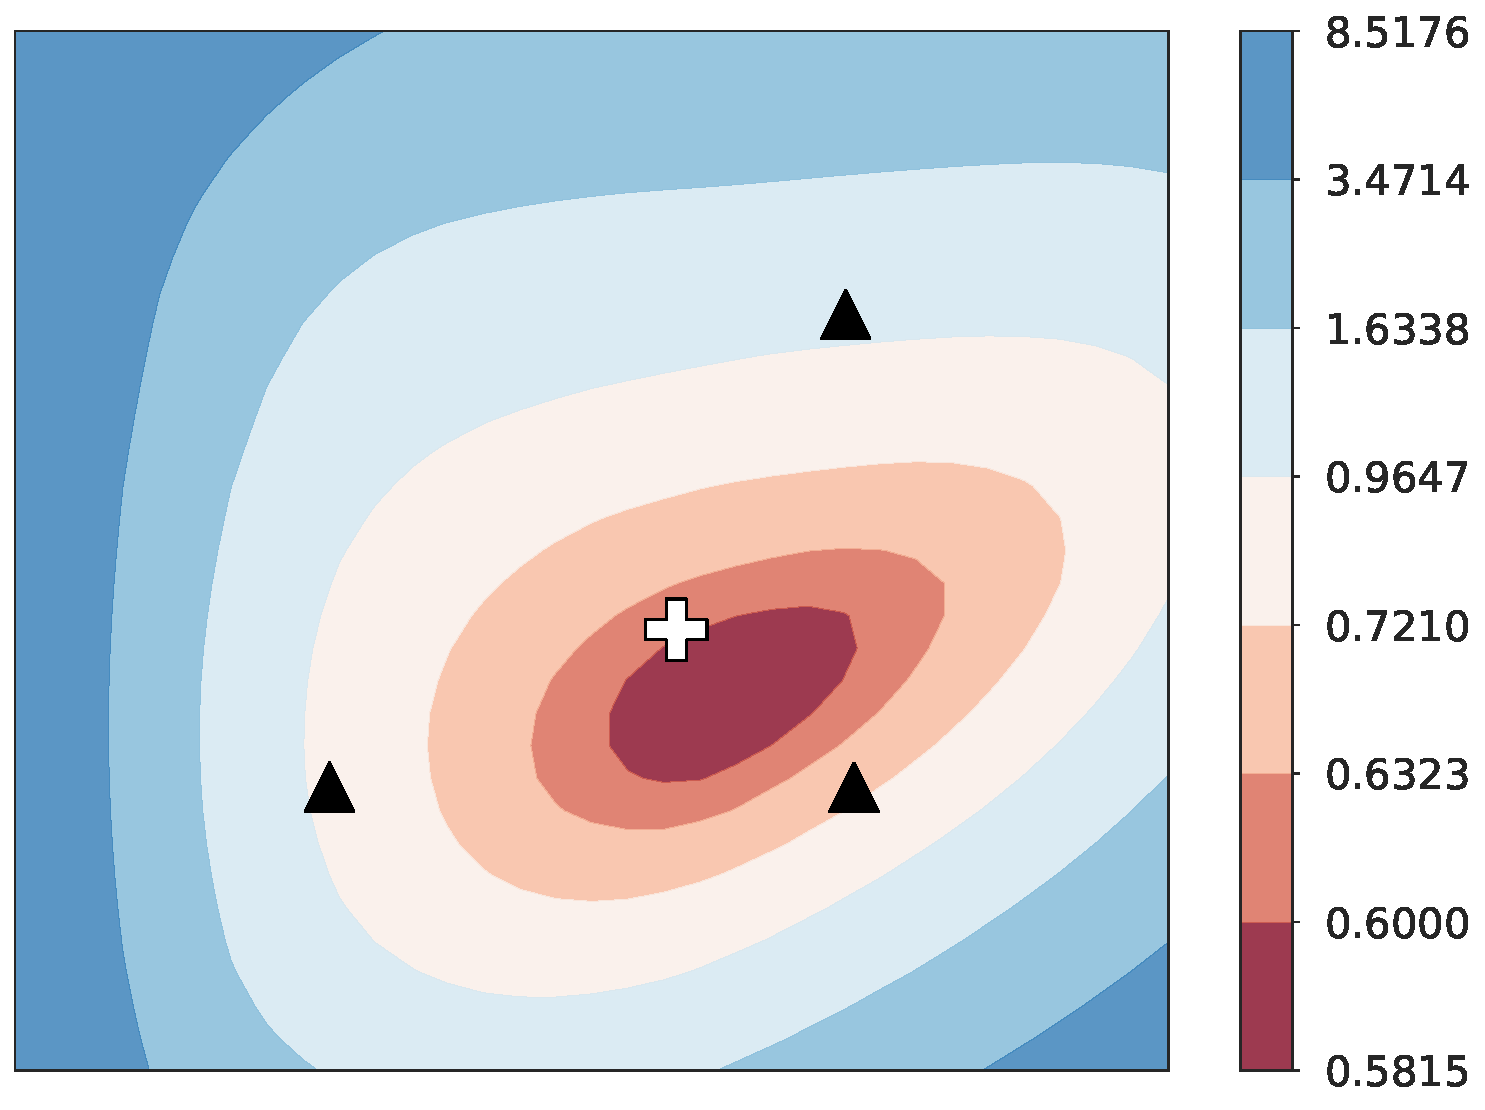
\includegraphics[width=\figwidth\textwidth]{figures/loss_surfaces/TE0_env0_in_loss_plane.pdf}}
    &
    \raisebox{-0.5\height}{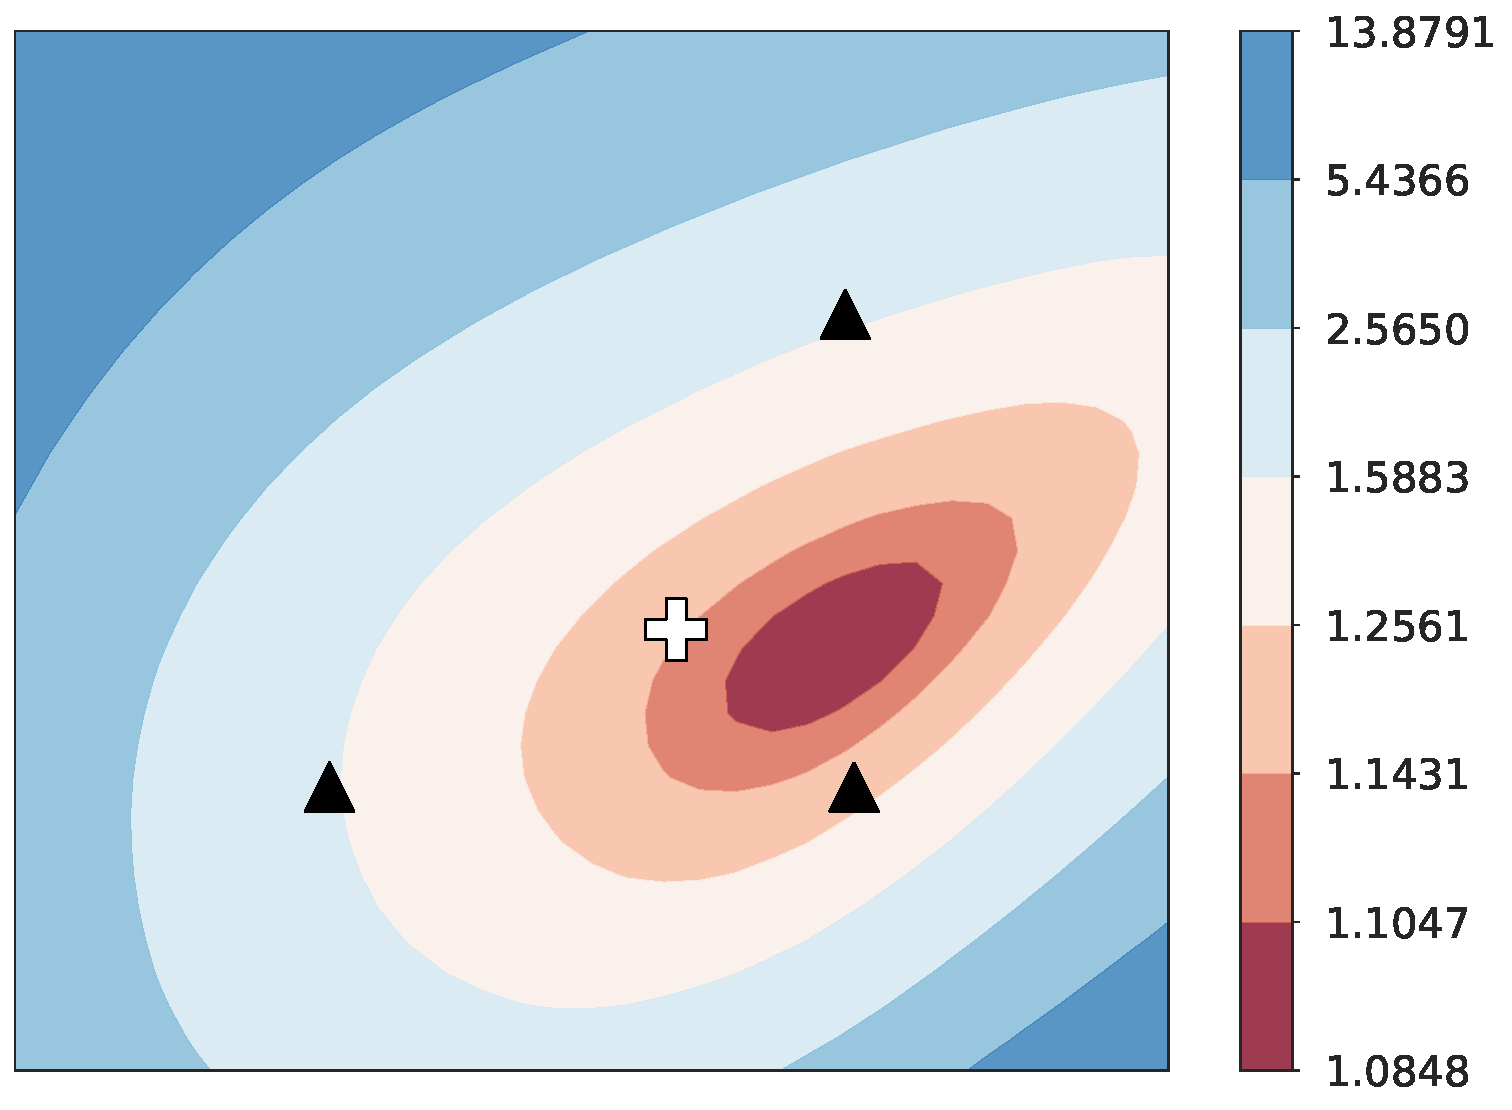
\includegraphics[width=\figwidth\textwidth]{figures/loss_surfaces/TE1_env1_in_loss_plane.pdf}}
    &
    \raisebox{-0.5\height}{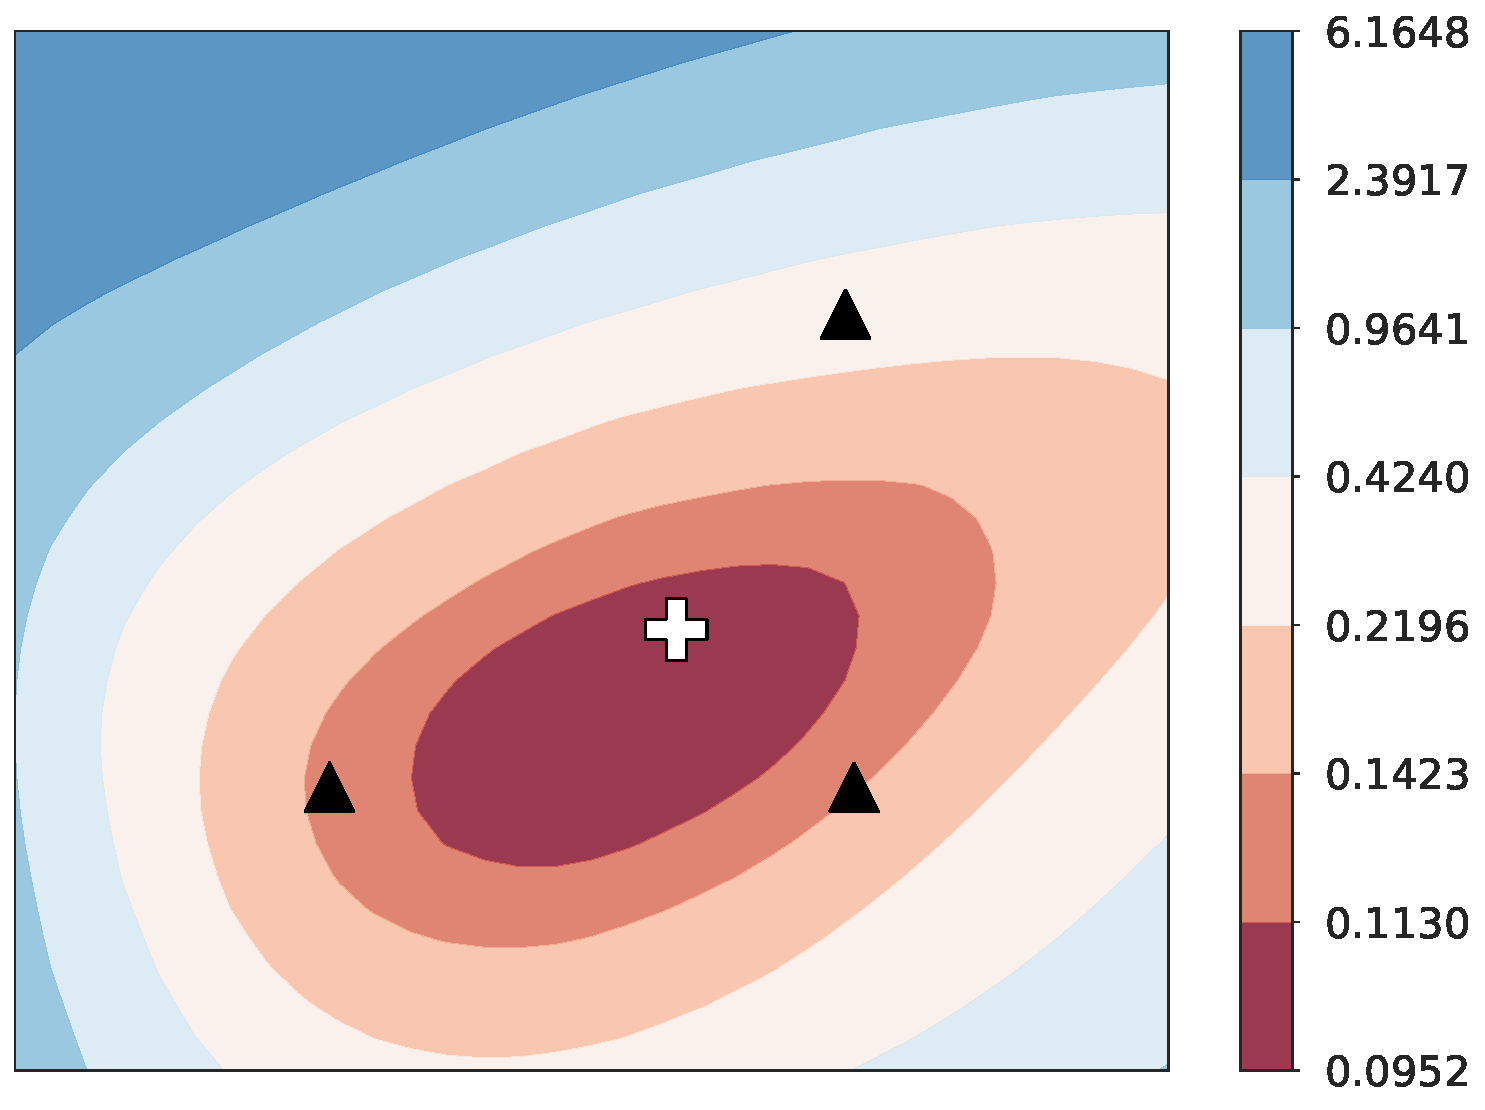
\includegraphics[width=\figwidth\textwidth]{figures/loss_surfaces/TE2_env2_in_loss_plane.pdf}}
    &
    \raisebox{-0.5\height}{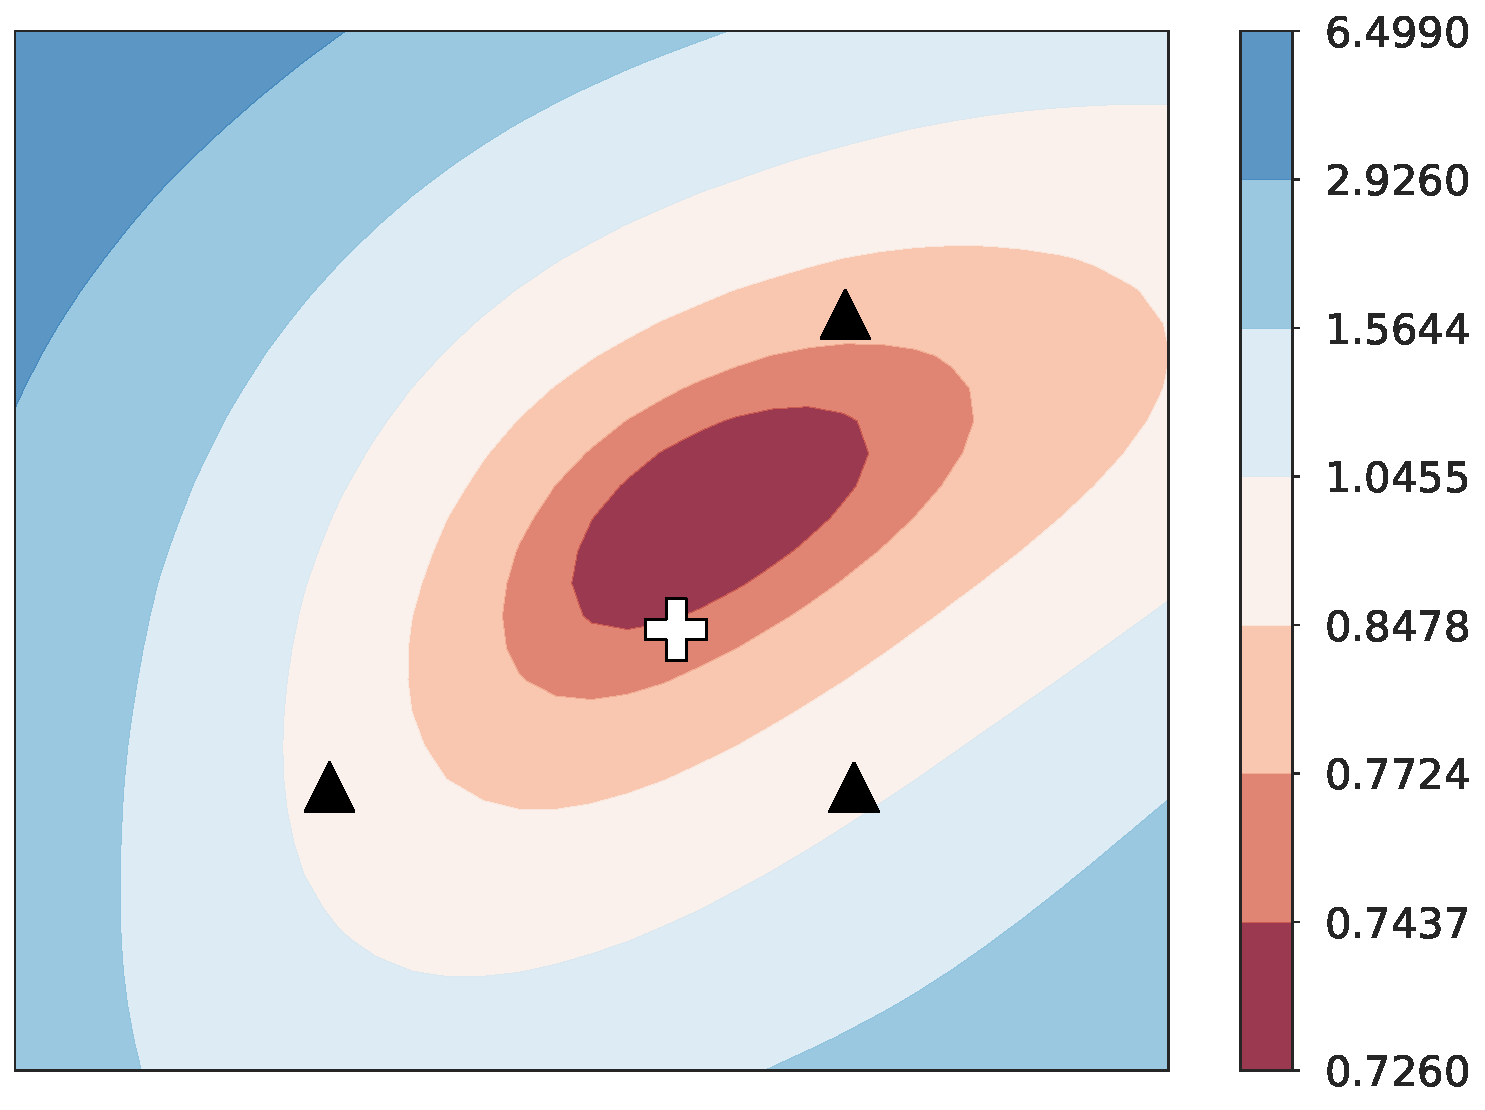
\includegraphics[width=\figwidth\textwidth]{figures/loss_surfaces/TE3_env3_in_loss_plane.pdf}}
\\
    &
    {\small \textit{Art painting} (test)}
    &
    {\small \textit{Cartoon} (test)}
    &
    {\small \textit{Photo} (test)}
    &
    {\small \textit{Sketch} (test)}
\end{tabular*}
%
\end{center}
\vspace{-0.5em}
\caption{\small \textbf{Loss surfaces on model parameters in \data{PACS} dataset for each target domain.} 
The three triangles indicate model weights chosen at the end of training phase with equal intervals. Each plane is defined by the three weights and losses upon the plane are visualized with contours. The center cross mark is averaged point of the three weights. The first and second rows show the averaged training loss and the test loss surfaces, respectively.
% \sr{coloring the center yellow?}
}
\vspace{-0.5em}
\label{fig:loss_space}
\end{figure}




% \iffalse

% % vertically centering
% \begin{figure*}[t]
% \centering
% %\raggedright
% \captionsetup[subfigure]{aboveskip=0pt,belowskip=0pt}
% \begin{subfigure}[b]{0.24\textwidth}
%     
\includegraphics[width=\textwidth]{figures/all_loss_surfaces/PACS/TE0_in_loss_plane.pdf}
%     % \caption{\textit{Art painting} (valid)}
% \end{subfigure}
% \begin{subfigure}[b]{0.24\textwidth}
%     
\includegraphics[width=\textwidth]{figures/all_loss_surfaces/PACS/TE1_in_loss_plane.pdf}
%     % \caption{\textit{Cartoon} (valid)}
% \end{subfigure}
% \begin{subfigure}[b]{0.24\textwidth}
%     
\includegraphics[width=\textwidth]{figures/all_loss_surfaces/PACS/TE2_in_loss_plane.pdf}
%     % \caption{\textit{Sketch} (valid)}
% \end{subfigure}
% \begin{subfigure}[b]{0.24\textwidth}
%     
\includegraphics[width=\textwidth]{figures/all_loss_surfaces/PACS/TE3_in_loss_plane.pdf}
%     % \caption{\textit{Photo} (test)}
% \end{subfigure}
% \\
% % \raggedright
% \begin{subfigure}[b]{0.24\textwidth}
%     
\includegraphics[width=\textwidth]{figures/all_loss_surfaces/PACS/TE0_env0_in_loss_plane.pdf}
%     \caption{\textit{Art painting} (test)}
% \end{subfigure}
% \begin{subfigure}[b]{0.24\textwidth}
%     
\includegraphics[width=\textwidth]{figures/all_loss_surfaces/PACS/TE1_env1_in_loss_plane.pdf}
%     \caption{\textit{Cartoon} (test)}
% \end{subfigure}
% \begin{subfigure}[b]{0.24\textwidth}
%     
\includegraphics[width=\textwidth]{figures/all_loss_surfaces/PACS/TE2_env2_in_loss_plane.pdf}
%     \caption{\textit{Photo} (test)}
% \end{subfigure}
% \begin{subfigure}[b]{0.24\textwidth}
%     
\includegraphics[width=\textwidth]{figures/all_loss_surfaces/PACS/TE3_env3_in_loss_plane.pdf}
%     \caption{\textit{Sketch} (test)}
% \end{subfigure}

% \vspace{-0.5em}
% \caption{\textbf{Loss surfaces on model parameters in \data{PACS} dataset for each target domain. 
% %In-distribution loss surface when target domain is \textit{photo} in PACS dataset.
% } 
% The three points such as circle, rectangle, and triangle indicate model weights chosen at the end of training phase with equal intervals. Each plane is defined by the three weights and losses upon the plane are visualized with contours. First and second rows show the averaged training loss and the test loss surfaces, respectively.\sr{put ``in-domain loss'' and ``out-of-domain loss'' on the left}}
% \vspace{-1.0em}
% \label{fig:loss_space}
% \end{figure*}

% \fi

\begin{figure}
\centering
    \begin{subfigure}{0.5\linewidth}
        
\includegraphics[width=\linewidth]{figures/accfluc/acc_fluc_legend.pdf}
    \end{subfigure}\\
    \begin{subfigure}{0.25\linewidth}
        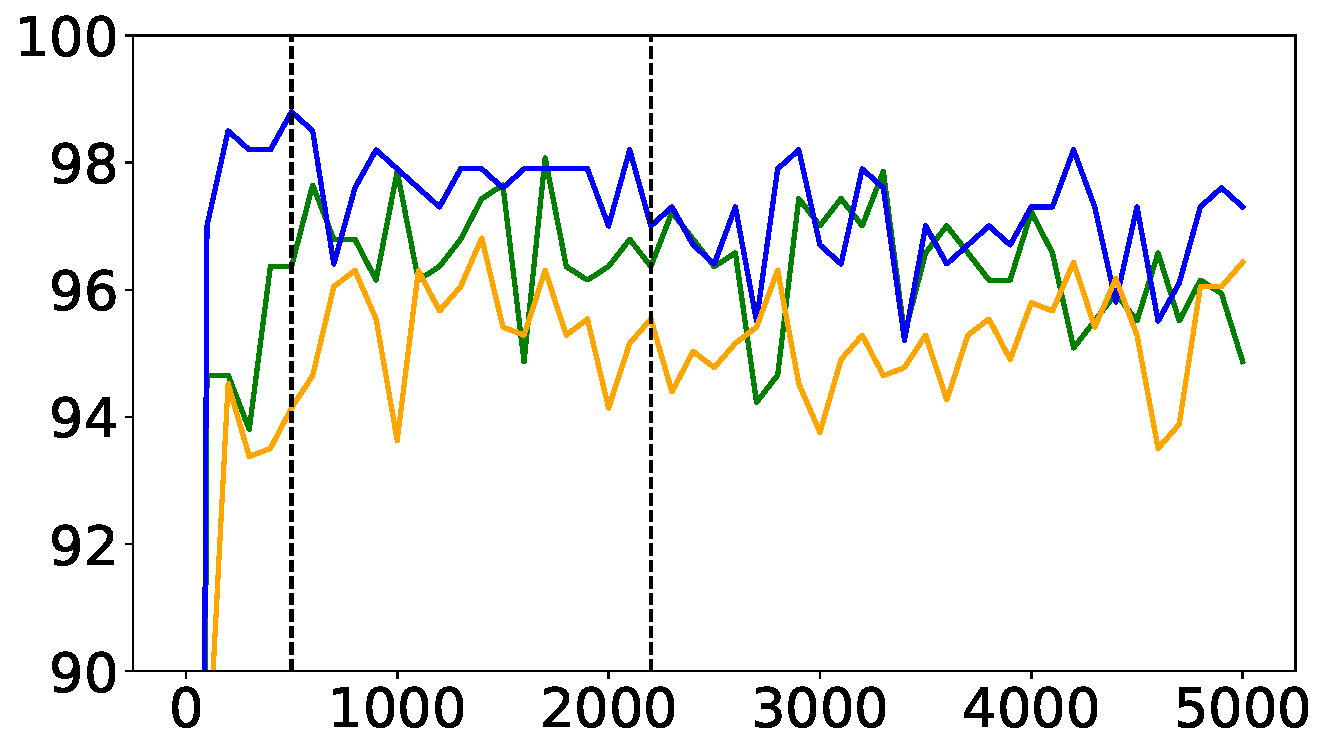
\includegraphics[width=\linewidth]{figures/accfluc/acc_fluc_TE0.pdf}%
        \caption{\small \textit{Art painting} (test)}
    \end{subfigure}%
    \begin{subfigure}{0.25\linewidth}
        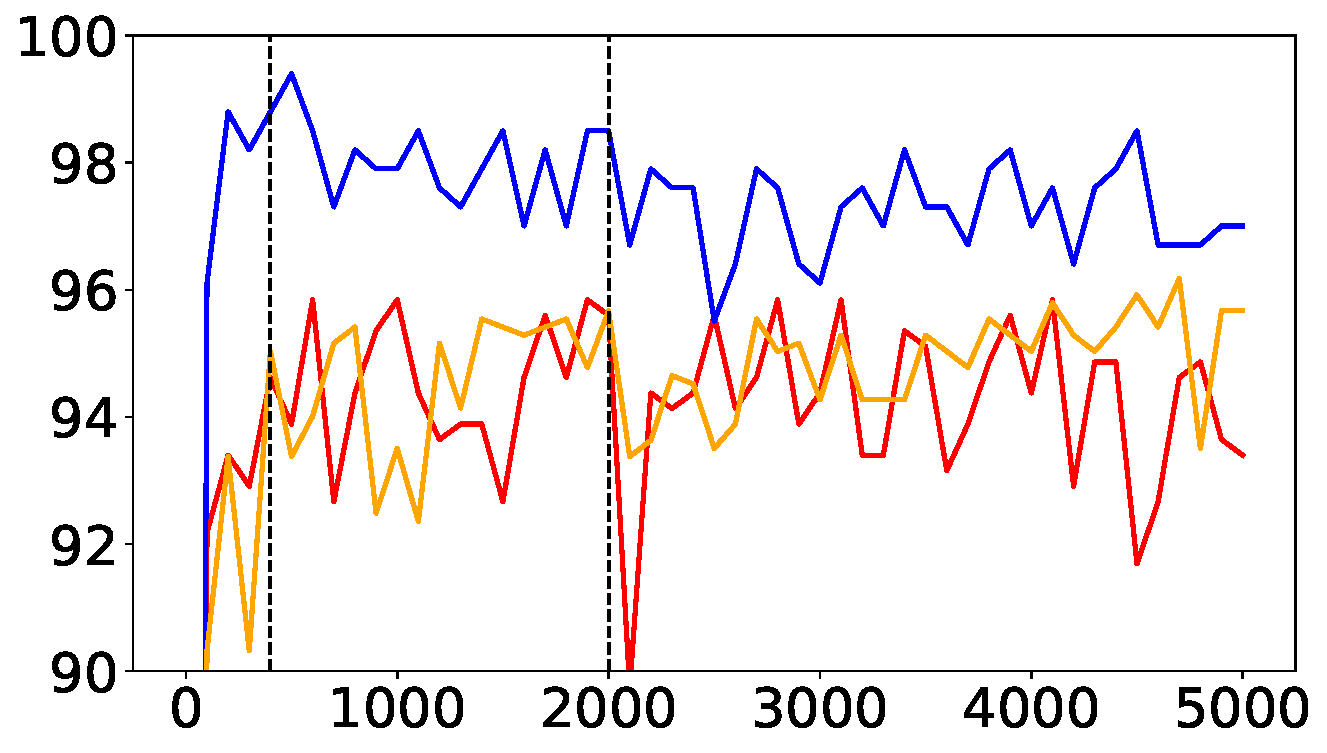
\includegraphics[width=\linewidth]{figures/accfluc/acc_fluc_TE1.pdf}%
        \caption{\small \textit{Cartoon} (test)}
    \end{subfigure}%
    \begin{subfigure}{0.25\linewidth}
        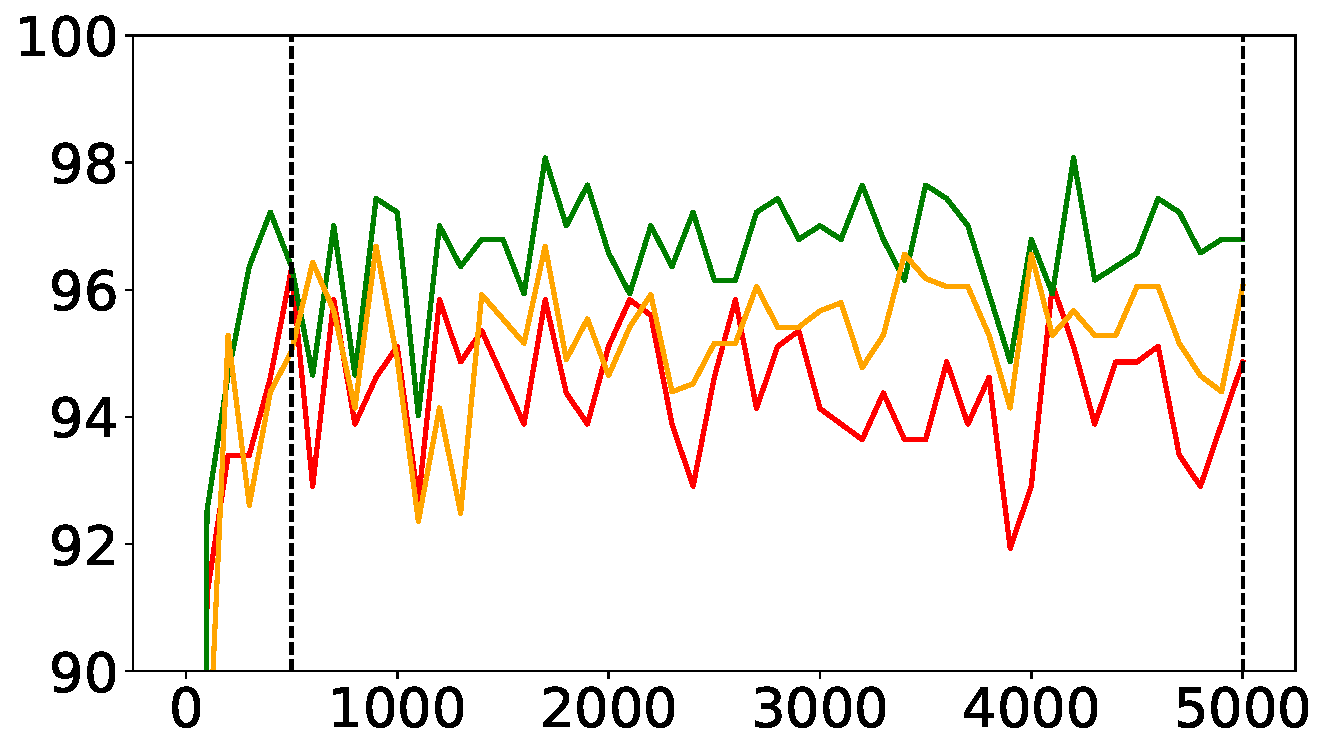
\includegraphics[width=\linewidth]{figures/accfluc/acc_fluc_TE2.pdf}%
        \caption{\small \textit{Photo} (test)}
    \end{subfigure}%
    \begin{subfigure}{0.25\linewidth}
        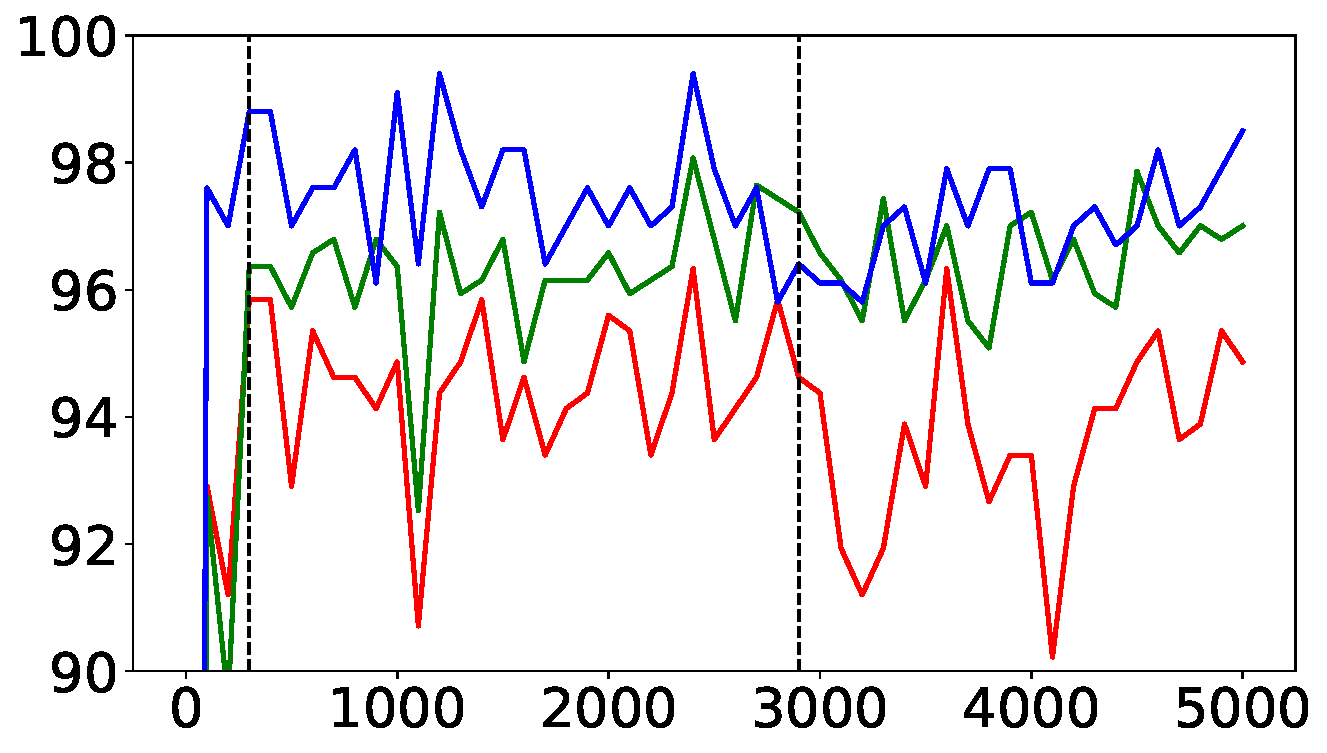
\includegraphics[width=\linewidth]{figures/accfluc/acc_fluc_TE3.pdf}%
        \caption{\small \textit{Sketch} (test)}
    \end{subfigure}%
    \caption{\small \textbf{Validation accuracies for in-domains.} The X- and Y-axis indicate the training iterations and accuracy, respectively, about the validation domains (legend) and the test domain (caption). The vertical dot lines represent start and end iterations, $t_s$ and $t_e$, identified by the overfit-aware sampling strategy of SWAD.}
    \label{fig:accfluc}
\end{figure}

\paragraph{Loss surface visualization.}
We visualize the loss landscapes by choosing three model weights on the optimization trajectory ($\theta_1, \theta_2, \theta_3$)\footnote{We choose weights at iteration 2500, 3500, 4500 during the training.}, and computing the loss values by linear combinations of $\theta_1, \theta_2, \theta_3$\footnote{Each point is defined by two axes $u$ and $v$ computed by $u=\theta_2 - \theta_1$ and $v=\frac{(\theta_3 - \theta_1)- \langle \theta_3 - \theta_1, \theta_2 - \theta_1 \rangle}{\|\theta_2 - \theta_1 \|^2 \cdot (\theta_2 - \theta_1)}$.} as \cite{izmailov2018swa}.
More details are in Appendix B.5.
In Figure~\ref{fig:loss_space}, we observe that for all cases, ERM solutions are located at the boundary of a flat minimum of training loss, resulting in poor generalizability in test domains, that is aligned with our theoretical analysis and empirical flatness analysis.
Since ERM solutions are located on the boundary of a flat loss surface, we observe that ERM solutions are very sensitive to model selection.
In Figure~\ref{fig:accfluc}, we illustrate the validation accuracies for each train-test domain combination of \data{PACS} by ERM, over training iterations (one epoch is equivalent to 83 iterations).
We first observe that ERM rapidly reaches the best accuracy within only a few training epochs, namely less than 6 epochs.
Furthermore, the ERM validation accuracies fluctuate a lot, and the final performance is very sensitive to the model selection criterion.

On the other hand, we observe that SWA solutions are located on the center of the training loss surfaces as well as of the test loss surfaces (Figure~\ref{fig:loss_space}). Also, our overfit-aware stochastic weight gathering strategy (denoted as the vertical dot lines in Figure~\ref{fig:accfluc}) prevents the ensembled weight from overfitting and makes SWAD model selection-free.